\section{Abstract}

This analysis is aimed at finding events coming from the decay $B_s^0 \to \psi (2S)K_S^0$ using a large data sample recorded by the LHCb experiment in Run 2. 
To identify and extract rare decay channels, an extensive analysis including machine learning methods is needed.
The extracted number of signal events is $n_\text{sig} = \num{45}$ and the number of background events is $n_\text{bkg} = \num{32}$, with a significance of $m = \num{5.1}$ in the signal region.

\section{Introduction}
The Standard Model (SM) of Particle Physics describes all fundamental interactions except for the gravitational force.
However, there are many phenomena such as the gravitational force, the enormous matter-antimatter asymmetry observed in the universe and the presence of
dark matter that cannot be properly explained. Hence, it is important to test the SM by means of precision measurements. In contrast to searches of New Physics (NP) through the
direct production in high-energy collisions, they can also be produced virtually in low-energy processes such as in hadronic decays involving beauty or charm quarks. Due to Heisenberg's uncertainty
principle, they can exist for a short period of time and contribute as quantum corrections, representing a complementary way of searching for NP indirectly. The Large Hadron Collider beauty (LHCb)
experiment investigates the differences between matter and antimatter by studying mesons containing charm and beauty quarks.\\
This analysis is aimed at using machine learning methods to extract rare signal events from a large data sample including $B_s^0 \to \psi (2S)K_S^0$ candidates recorded during Run 2 of the LHCb experiment. The decay 
channel $B_s^0 \to \psi (2S)K_S^0$ is a very rare decay, resulting in the data being dominated by combinatorial background and more common decays, which have been recorded due to trigger criteria being wrongly fulfilled.
To identify and extract these rare signal events, an extensive analysis including machine learning methods is needed.\\
The used data has been recorded uring Run 2 (2015-2018) of the LHCb experiment at CERN, proton bunches with a centre of mass energy of $\qty{13}{\tera\electronvolt}$ collided approximately $40 \times 10^6$ times per second~\cite{LHCb_MVA}.
The theoretical framework will be presented in \autoref{sec:Theorie}, followed by a description of the LHCb experiment in \autoref{sec:Detector}. The analysis strategy is presented in \autoref{sec:strategy}, followed by
the study of the dataset and the training of the machine learning model in \autoref{sec:Analysis}. The final results are summarized in \autoref{sec:Discussion}.
\newpage
\section{Theory}
\label{sec:Theorie}

Before diving into the analysis, one has to understand the underlying kinematics of the decay. The $B_s^0$ meson consists of a $s$ and a $\bar{b}$ quark (next to other sea quarks and gluons) and hence
has a neutral net electric charge. As for this decay channel, the $b$ quark of the $B_s^0$ meson interacts with a $W^+$ gauge boson and results in a charm pair $c \bar{c}$ and a $\bar{d}$ quark in the 
final state. Together with the strange quark from the $B_s^0$ meson, the final state consists of a $\psi (2S) \, [c \bar{c}]$ meson and a $K_S^0$ ("k-short") being a superposition of $d\bar{s}$ and $\bar{d}s$.
This decay can only occur via the weak force, since the quark flavour changes from $\bar{b}$ to $\bar{d}$. The Feynman diagram depicting this process is shown in \autoref{fig:Feynman_dia}.
\begin{figure}
    \centering
    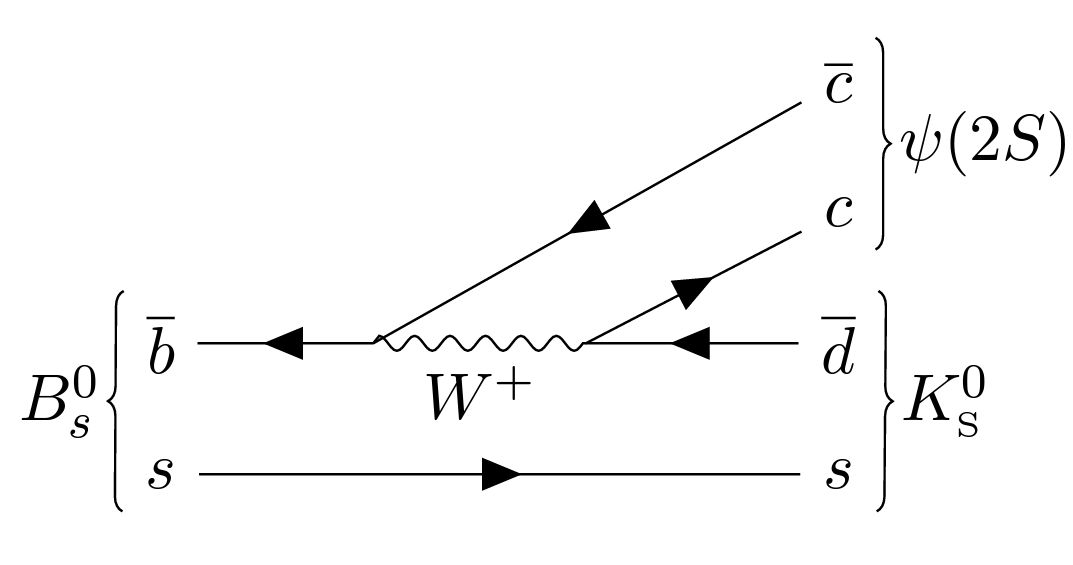
\includegraphics[width = .5\textwidth]{"content/pics/Feynman.png"}
    \caption{Feynman diagram of $B_s^0 \to \psi (2S)K_S^0$ \cite{LHCb_MVA}.}
    \label{fig:Feynman_dia}
  \end{figure}
\\The $\psi (2S)$ and $K_S^0$ are not directly detected in the detector. While $\psi (2S)$ mainly decays via strong interactions, it also decays via
electromagnetic force into a lepton pair ($l^+l^-$).
Since the detector has a good efficiency for detecting muons, only muon pairs will be regarded ($\mu^+\mu^-$). Due to the conservation of energy and momentum, the 
total mass of the muon pair is approximately equal to the mass of the $\psi (2S)$ meson. Due to energy conservation, the total mass of the muon is exactly equal due to the 
mass of the $\psi (2S)$ meson, but due to the limited detector resolution, the masses might differ to some extend. With cuts on the muon pair masses, the collected data is reduced to less signal candidates while
rejecting charm resonances $c\bar{c}$.\\
The dominant decay channel of $K_S^0$ is a pair of pions ($\pi^+\pi^-$) via weak interaction. The $K_L^0$ meson also consists of the superposition of $d\bar{s}$ and $\bar{d}s$ and has the same decay channels.
However, the branching fraction of that decay channel is two magnitudes smaller than for the $K_S^0$ and will therefore not interfere with the relevant signal candidates to a significant level. The mass and other
kinematic variables of the $K_S^0$ can be reconstructed with the produced pion pairs.\\
The given recorded data consists of various variables including kinematic properties of the muons, pions as well as the reconstructed $\psi (2S)$ and $K_S^0$ mesons. The $B_s^0$ can be reconstructed using the
properties of the $\psi (2S)$ and $K_S^0$ while using their true invariant masses, being $m_{\psi (2S)} = \qty{3686.097(0.011)}{\mega\electronvolt}$ and $m_{K_S^0} = \qty{497.611(0.013)}{\mega\electronvolt}$ \cite{PDG}.\\
The recorded data set does not only include $B_s^0 \to \psi (2S)K_S^0$ signal. Moreover, it primarily contains combinatorial background, consisting of random tracks mimicking the signal. 
The much more abundant decay $B^0 \to \psi (2S)K_S^0$ is also included in the recorded data. To differentiate between background and signal, an extensive analysis including
training a classifier is needed.\\
To evaluate and optimize the classifier (maximizing the number of signal candidates while keeping the background low), a loss function is to be minimized. The inverse of such loss functions is called figure of merit (FOM).
In this analysis, the Punzi figure of merit for optimizing the signal efficiency
\begin{equation}
    \label{eq:FOM}
    \mathrm{FOM}  = \frac{\epsilon_{\mathrm{sig}}}{5/2 + \sqrt{N_{\mathrm{bkg}}}}
\end{equation}
is to be maximized with $N_{\mathrm{bkg}}$ being the background candidates in the signal region (combinatorial background + $B^0 \to \psi (2S)K_S^0$ events) and $\epsilon_{\mathrm{sig}}$ being the efficiency of classifying
the signal. The signal efficiency is calculated by using a Monte Carlo simulation of $B_s^0 \to \psi (2S)K_S^0$. The BDT cannot discriminate between $B_s^0$ and $B_d^0$ events, due to the similarity of kinematic
properties. However, the resolution of the LHCb detector is well enough, to distinguish between the two decays in the mass spectrum after removing most background candidates.\\
To train an efficient and well performing classifier, the right choice of variables is needed. One has to look for those variables, which differ the most for background and signal. To find these, one can caluclate the 
largest distance between the cumulative probability distributions $F^i$ of these variables:
\begin{equation}
    \label{eq:Kolmogorov}
    \sup\limits_{n} | F_n^1 - F_n^2 |,
\end{equation}
with the index n running over all bins of the distributions.\\
The final result can be evaluated using the significance, being the number of signal candidates devided by the total number of events in the signal region, including background and signal.
It can be calculated by
\begin{equation}
    \label{eq:sign}
    m = \frac{N_{\mathrm{sig}}}{\sqrt{N_{\mathrm{sig}} + N_{\mathrm{bkg}}}},
\end{equation}
using the given number of signal and background candidates by the classifier. The significance is a quantity to measure of how likely the result is produced by statistical fluctuations.
